\section{Introduction}
The model which was used in \autoref{sec:PredictSign} was trained with a lot of images. To obtain training images, the \textbf{Gazebo} based simulation of OttoCar was used.

\section{Steps to produce training data}
\begin{enumerate}
    \item Each marking was placed on the track of the simulation numerous times as shown below.
    \label{enum:StepsToTrainingData1}
    \begin{figure}[h!]
    \begin{subfigure}{0.5\textwidth}
    \centering
    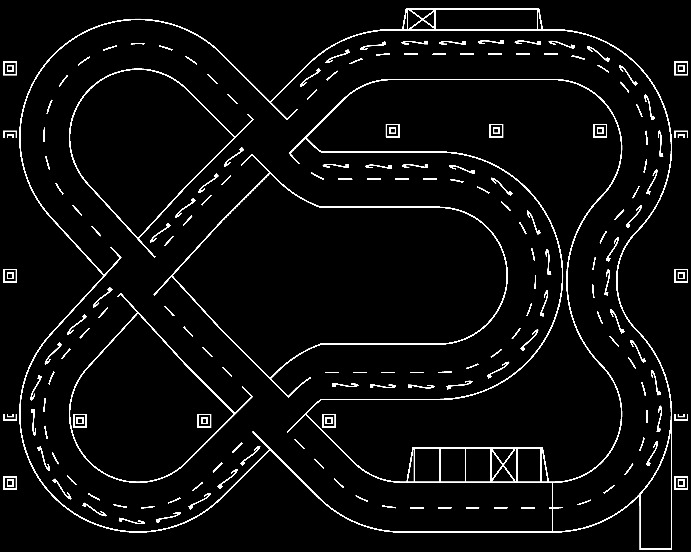
\includegraphics[scale=1]{images/SingleNumberOnTrack.png} 
    \caption{Markings of single number on track}
    \end{subfigure}
    \begin{subfigure}{0.5\textwidth}
    \centering
    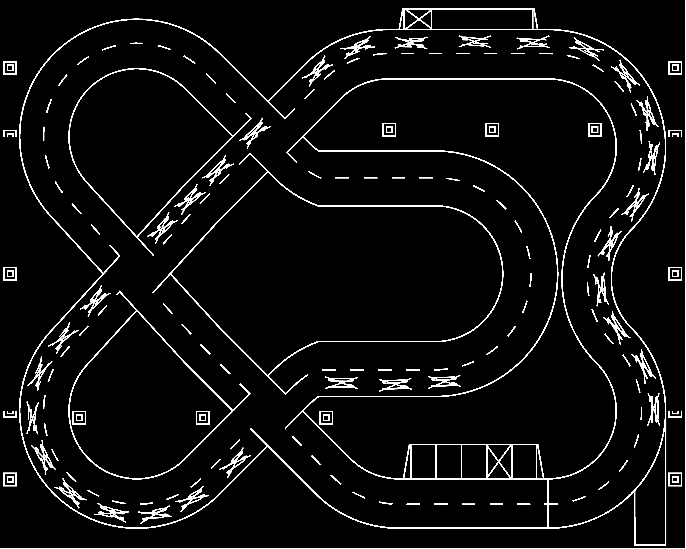
\includegraphics[scale=1]{images/SpeedEndOnTrack.png} 
    \caption{Markings of speed end on track}
    \end{subfigure}
    \caption{Marking signs on track for training data}
    \label{fig:SignsOnTrackForTrainingData}
    \end{figure}
    \item Simulation was run and the top view images generated were saved at 30 frames per second.
    \item The images of markings were processed and extracted from the saved top view images as mentioned in the steps of image processing. These 20 x 20-pixel images were saved.
    \label{enum:StepsToTrainingData3}
    \item Repeat \hyperlink{enum:StepsToTrainingData1}{Step 1} to \hyperlink{enum:StepsToTrainingData1}{Step 3} for all the markings. There is a total of 13 classes and around 1000 training images were generated for each class.
    \item The training images obtained were checked for images not containing a valid marking and invalid images were deleted.
    \item Class labels are assigned to the training images.
    \item The training images were split into 80\% training and 20\% testing.
    \item HOG features of the images were computed using the parameters:
    \begin{itemize}
        \item winSize = (20,20)
        \item blockSize = (10,10)
        \item blockStride = (5,5)
        \item cellSize = (10,10)
        \item nbins = 9
    \end{itemize}
    \item An SVM model using Radial Basis Function as kernel is set up in OpenCV.
    \item OpenCV API provides an auto train function to train SVM classifier without specifying the hyper parameters. It does the training multiple times and chooses the optimal hyper parameters.
Auto train function was used to train the SVM classifier.
    \item Using the test dataset the trained classifier was evaluated. An accuracy of 99\% was obtained.
    \item The trained model was saved as \emph{svm\_data.dat} file.
\end{enumerate}